\documentclass[11pt, oneside]{article}   	

%%%%%%%%%%%%%%%%%%%%%%%%%%%%%%%%%%
% Packages
%%%%%%%%%%%%%%%%%%%%%%%%%%%%%%%%%%
\usepackage[colorlinks,citecolor=blue,urlcolor=blue,filecolor=blue,backref=page]{hyperref}

\usepackage{geometry}                	
\geometry{a4paper}                   	

\usepackage{graphicx}	
\usepackage{float}
\usepackage{subfig}
\usepackage{afterpage}

\usepackage{amsthm}
\usepackage{amsmath}							
\usepackage{amssymb}
\usepackage[utf8]{inputenc}

\usepackage{natbib}

\usepackage{url}

\usepackage{commath}

%%%%%%%%%%%%%%%%%%%%%%%%%%%%%%%%%%
% Macros
%%%%%%%%%%%%%%%%%%%%%%%%%%%%%%%%%%

\newcommand{\thetab}{{\boldsymbol{\theta}}}
\newcommand{\thetaHat}{{\hat{\thetab}}}
\newcommand{\alphab}{{\boldsymbol{\alpha}}}
\newcommand{\betab}{{\boldsymbol{\beta}}}
\newcommand{\mub}{\boldsymbol{\mu}}
\newcommand{\Sigmab}{\boldsymbol{\Sigma}}
\newcommand{\xib}{{\boldsymbol{\xi}}}
\newcommand{\xitildeb}{{\boldsymbol{\tilde{\xi}}}}
\newcommand{\pnorm}{p}
\newcommand{\pnn}{\phi}
\newcommand{\pnnj}{f}
\newcommand{\pdata}{p_{ \mathbf x}}
\newcommand{\pnoise}{p_{ \mathbf y}}
\newcommand{\pcondnoise}{p_{\y|\x}}
\newcommand{\palpha}{p_\alphab}
\newcommand{\pbeta}{p_\betab}
\newcommand{\q}[1]{q(\z|{#1})}

\newcommand{\Ib}{\boldsymbol{I}}
\renewcommand{\u}{{\mathbf u}}
\newcommand{\x}{{\mathbf x}}
\newcommand{\y}{{\mathbf y}}
\newcommand{\z}{{\mathbf z}}
\newcommand{\w}{{\mathbf w}}
\newcommand{\ytilde}{\mathbf{\tilde{y}}}
\newcommand{\X}{{\mathbf X}}
\newcommand{\psib}{\boldsymbol{\psi}}


\renewcommand{\P}{\mathbb{P}}
\newcommand{\E}{\mathbb{E}}
\newcommand{\Ex}{\E_{\x}}
\newcommand{\Ey}{\E_{\y}}
\newcommand{\Evar}[1]{\E_{\z \sim \q{#1}}}
\newcommand{\Ealpha}{\mathbb{E}_{\alphab}}
\newcommand{\Ebeta}{\mathbb{E}_{\betab}}

\newcommand{\J}{\mathcal{J}}


%%%%%%%%%%%%%%%%%%%%%%%%%%%%%%%%%%
% Latex settings
%%%%%%%%%%%%%%%%%%%%%%%%%%%%%%%%%%

\graphicspath{{./figs/}}


%%%%%%%%%%%%%%%%%%%%%%%%%%%%%%%%%%
% Text
%%%%%%%%%%%%%%%%%%%%%%%%%%%%%%%%%%

\title{Interim Report: Noise Contrastive Estimation with Unobserved Variables}
\author{Ben Rhodes}
\date{\today}						

\begin{document}
\maketitle

\section{Introduction}

This thesis presents a method for estimating the parameters of unnormalised probability densities with unobserved (or `latent’) variables. The method is an extension of noise-contrastive estimation, which applies only to unnormalised, fully observed models. Before introducing the method, it helps to first understand the definitions and difficulties of both unnormalised and latent variable models.

An unnormalised model, $\pnn(\u;\thetab)$, is a parametrised family of functions that you can think of as scaled probability density \footnote{unless stated otherwise, assume that all results apply equally to probability mass functions defined over discrete random variables, replacing integrals with sums as necessary.} functions that do not integrate to 1 for all values of $\thetab$. That is:
 \begin{align}
   \int_{\u }\pnn(\u;\thetab) \dif \u &= Z(\thetab) \neq 1 & \pnn(\u;\thetab) \geq 0
\label{eq:Zdef}
  \end{align}
where $Z(\thetab$) is called the \emph{partition function}. The partition function is important because it allows us to normalise $\pnn(\u;\thetab)$, obtaining a model $\pnorm(\u; \thetab)$ that, regardless of the value of $\thetab$, integrates to 1.
\begin{align}
  \pnorm(\u;\thetab)&=\frac{\pnn(\u;\thetab)}{Z(\thetab)}, & \int_{\u }\pnorm(\u;\thetab) \dif\u & = 1.
  \label{unnormalised density}
\end{align}
Unfortunately, the partition function is rarely computable analytically, and the cost of approximating it numerically scales exponentially in general. The intractability of the partition function becomes problematic when we want to estimate good values of $\thetab$ given some data $\{\x_1, ..., \x_n\}$, where `good' - in practical terms - means that  $\pnorm(\x_i; \thetab)$ is large for all $i$ (whilst still satisfying the constraint of integrating to 1). It is problematic because the standard approach of maximum likelihood estimation requires us to maximise an objective that depends on the partition function; namely, the log-likelihood:
\begin{align}
\ell(\thetab) &= \Ex \left( \log \pnorm(\x;\thetab) \right) = \Ex \left( \log \pnn(\x;\thetab) \right) - \log ( Z(\thetab) ),
\label{eq:log-likelihood}
\end{align}
In light of this intractability, significant work has gone into building estimators that avoid directly computing the partition function, such as pseudolikelihood \citep{besag1975statistical}, score matching \citep{hyvarinen2005estimation}, ratio matching \citep{hyvarinen2007some}, contrastive divergence \citep{hinton2006training}, persistent contrastive divergence \citep{younes1998stochastic, tieleman2009using} and noise-contrastive estimation \citep{gutmann2012noise}. It is this final method, noise-contrastive estimation, that we build on this thesis, extending its applicability to latent variable models. 

A latent variable model is a family of probability densities $\pnorm(\u; \thetab)$ for which we do not have a direct expression; instead we only have a joint $\pnorm(\u, \z; \thetab)$ density, where $\z$ are hidden variables, not present in our data set. We thus obtain $\pnorm(\u; \thetab)$ only after marginalisation:
\begin{align}
  \pnorm(\u; \thetab) = \int \pnorm(\u, \z;\thetab) \dif \z
  \label{eq:marginal}
\end{align}

Learning the parameters $\thetab$ is problematic here for essentially the same reason as in normalised models: the presence of an intractable integral. In section \ref{sec:variational NCE} we discuss a general strategy for overcoming this intractability using variational inference.

To see why latent variable models are important, it helps to consider two conceptually distinct (but mathematically equivalent) types of latent variables. The first type represent `missing data’; perhaps certain pixels in an image were corrupted, generating NaNs. The second type represent compressions of the visible data, which often (but not always) capture low-dimensional causes of the visible data. Such compressions are at the core of unsupervised learning, since the ability to build parsimonious models of the hidden causes of your observations appears to be a fundamental aspect of intelligence. Thus, it is primarily the second view of latent variables that motivates the widespread use of such models. 

Let us now consider the combined case of an unnormalised, latent variable model. To write down an expression for $\pnorm(\u; \thetab)$, we combine equations \ref{unnormalised density} and \ref{eq:marginal} to get:
\begin{align}
    \pnorm(\u; \thetab) = \frac{\int \pnn(\u, \z;\thetab) \dif \z}{Z(\thetab)}
\end{align}
where $Z(\thetab)$ is as we defined it in equation \ref{eq:Zdef}. This expression contains two troublesome integrals, and it is this double intractability that is the fundamental technical barrier we must overcome to perform parameter estimation.

Of course, there is no use solving this problem if such models are not useful. Fortunately, this is not the case. Unnormalised, latent variable models arise naturally in the context of undirected graphical models (or ‘Markov networks’) \citep{kindermann1980markov} which are very general tools for describing probabilistic relations between random variables. An exemplary case is the Restricted Boltzmann Machine (RBM) \citep{smolensky1986information} which is treated in section \ref{sec:rbm}. The dominant approach to learning in models such as an RBM is to use a variant of contrastive divergence. However, there are some theoretical and empirical reasons to prefer noise-contrastive estimation to contrastive divergence \citep{gutmann2012noise} in the case of fully observed models, and so we might expect the same to be true in the latent variable case. Investigating this claim is one of principal goals of this thesis.




\section{Background}
\subsection{Noise-contrastive estimation}
\label{sec:nce}
NCE converts an unsupervised density estimation problem into a supervised classification problem, by training a (non-linear) logistic classifier to distinguish between the true data and samples from some reference distribution, which we refer to as noise samples.

Concretely, we first generate $m$ samples $\{\textbf{y}_1, \ldots \textbf{y}_m\}$ from a noise distribution $\pnoise(\textbf{y})$ and mix these samples with our data $(\textbf{x}_1, …., \textbf{x}_n)$. Our goal is now to classify whether a random sample $\u$ from this mixture came from the data-generating distribution $p$ or the noise $\pnoise$. We do so by calculating posterior probabilities, using our unnormalised model $\phi(\u; \thetab)$ as a surrogate for the true probability of the data $p(\u)$. If $\nu = \frac{m}{n}$, then:
\begin{align}
    \P( \u \sim \pdata; \thetab ) &= \frac{\pnn(\textbf{u}; \thetab)}{\pnn(\textbf{u}; \theta) + \nu \pnoise(\textbf{u})} = 
    \frac{1}{1 + \nu \exp \left( -h(\u;\thetab) \right)} \label{eq:nce prob data}\\
    \P( \u \sim \pnoise; \thetab ) &= \frac{\pnoise(\textbf{u})}{\frac{1}{\nu}\pnn(\textbf{u}; \theta) + \pnoise(\textbf{u})} = 
    \frac{1}{1 + \frac{1}{\nu} \exp \left( h(\u;\thetab) \right)} \label{eq:nce prob noise} \\
\end{align}
where:
\begin{align}
    h(\u;\thetab) = \log \pnn(\u ; \thetab) - \log \pnoise(\textbf{u})
\end{align}
At first, the rightmost expressions in \ref{eq:nce prob data} and \ref{eq:nce prob noise} may appear unnecessary, but if we absorb the $\nu$ terms into the exponentials, then we see that the probabilities of each class (data or noise), is expressed with a sigmoid. Our classification problem can therefore be thought of as a (non-linear) logistic regression problem, with objective function:
\begin{align}
  J_n(\thetab)&= \frac{1}{n} \left\{\sum_{i=1}^{n} \log  \P( \x_i \sim \pdata; \thetab ) + \sum_{i=1}^{m} \log\left[\P( \y_i \sim \pnoise; \thetab )\right]\right\}\\
  & = -\frac{1}{n} \left\{\sum_{i=1}^{n} \log \left[1+\nu \exp(-h(\x_i;\thetab))\right] + \sum_{i=1}^{m} \log \left[1+ \frac{1}{\nu} \exp(h(\y_i;\thetab))\right]\right\}
  \label{eq:Jn}
\end{align}
which is the sample version of $J(\thetab)$,
\begin{equation}
  J(\thetab) = - \Ex  \log \left[1+\nu \exp(-h(\x;\thetab))\right] - \nu \Ey \log \left[1+1/\nu \exp(h(\y;\thetab))\right]
  \label{eq:J}
\end{equation}

If we assume that the true data generating distribution is $\pnorm(\u; \thetaHat)$, and that this distribution is contained within our unnormalised family $\phi(\u;\thetab)$, then optimising the above objective function guarantees that $\thetab$ converges (in probability) to $\thetaHat$ in the limit of infinite data.

Why should the \emph{normalised} data generating distribution live in an \emph{unnormalised} family? This assumption may seem odd at first, but note that it is simple to give the model family $\pnn(\u; \thetab)$ an extra degree of freedom by multiplying it with a scaling parameter $c$. This new parameter is estimated in conjunction with $\thetab$, so that we automatically obtain a normalised solution. \footnote{note, this is \emph{not} the same as normalising the model i.e computing the partition function, which provides the normalisation constant for \emph{every} value of $\thetab$}

It turns out that for $\nu$ sufficiently large, the choice of noise distribution $q$ is not important. However, increasing $\nu$ uses more computational resource, so we still need to select an appropriate distribution. It remains an area of active research to select $\pnoise$ based on theoretically justified properties, with the main constraints currently being that it should be cheap to sample from, non-zero wherever $\pnn$ is non-zero, and similar to the underlying the data generating distribution.

In the case of latent variable models, the extended version of NCE that we present in this thesis is able to partially automate the construction of a suitable noise distribution, which is a significant advance over hand-crafted choices.




\subsection{Variational lower bound on NCE objective function}
\label{sec:variational NCE}
Guttmann [2018, unpublished] derived a \emph{variational} lower bound to the NCE objective function, which is the mathematical keystone to this thesis. Before presenting the bound, we first give a more standard introduction to the variational approach, which should make the subsequent material clearer.

When learning the parameters of normalised models, it usually makes sense to use the log-likelihood objective function given in equation \ref{eq:log-likelihood}. In the presence of latent variables, the log-likelihood becomes:
\begin{align}
    \ell(\thetab) &= \Ex \left( \log \left( \int \pnorm(\x, \z;\thetab) \dif \z  \right) \right) \\
                  &= \Ex \left( \log \left( \Evar{\x} \left( \frac{\pnorm(\x, \z;\thetab)}{\q{\x}} \right)  \right) \right)
\end{align}
where, in the second line, we applied a simple identity known as importance sampling, where the `auxiliary' density $q$ can be any valid density that is non-zero whenever $\pnorm$ is non-zero. We then apply Jensen's inequality, using the fact that the $\log$ function is concave, giving:
\begin{align}
    \ell(\thetab) &\geq \Ex \Evar{\x} \left( \log \left( \frac{\pnorm(\x, \z;\thetab)}{\q{\x}} \right) \right)
    \label{eq:elbo}
\end{align}
It is straightforward to show that this inequality is tight when $\q{\x} = \pnorm(\z | \x; \thetab)$. This inequality directly leads to an iterative algorithm, known as Expectation Maximisation (EM) for estimating the parameters $\thetab$. Whilst the idea of EM is quite old, originating from \citep{dempster1977maximum}, the view presented here is similar to \citep{neal1998view}. The algorithm simply involves alternating between optimising the right-hand side of equation \ref{eq:elbo} with respect to $\thetab$ (which we can do since we have an expression for $\pnorm(\x, \z;\thetab)$) and then, with our new $\thetab$, setting: $\q{\x} = \pnorm(\z | \x; \thetab)$. One can prove that this iterative algorithm always increases the log-likelihood.

EM, as stated above, assumes we have an expression for $\pnorm(\z | \x; \thetab)$. That is, we assume \emph{inference} of the latent variables is tractable. What if this is not the case? Well, we still want $q$ to approximate the posterior over latent variables, and so we could parametrise it with parameters $\alphab$. If this parametric family is sufficiently broad, we might hope that one of its members is close to the true posterior, and that we can find such a member by optimising $\alphab$. Thus, instead of resetting: $\q{\x} = \pnorm(\z | \x; \thetab)$, we optimise the right-hand side of \ref{eq:elbo} with respect to the \emph{variational parameters} $\alphab$.

How to perform this optimisation with respect to $\alphab$ is a matter of ongoing research. It is non-trivial because the right-hand side of $\ref{eq:elbo}$ involves an expectation with respect to $q(\z|\x; \alphab)$, so standard gradient-based methods are hard to straightforwardly apply. There are methods to cope with this obstacle, such as the reparameterisation trick \citep{kingma2015variational}, which we discuss in later chapters. 

This concludes the standard application of variational inference to the log-likelihood objective function. The question remains, how can we apply a similar strategy to the NCE objective function in equation \ref{eq:J}? There are two fundamental steps: 
\begin{itemize}
    \item Use importance sampling to re-express the intractable integral over $\z$ as an expectation; call this E.
    \item Apply Jensen’s inequality to a concave function g(E).
\end{itemize}
One complication in applying such a strategy is that the intractable integral $\int \pnn(\u, \z;\thetab) \dif \z$ appears twice: inside the expectation with respect to the data:
\begin{align}
    - \Ex  \log \left[1+\nu \exp(-h(\x;\thetab))\right]
    \label{eq:J term1}
\end{align}
and it also appears in the second term, which is an expectation with respect to the noise distribution:
\begin{align}
    - \nu \Ey \log \left[1+1/\nu \exp(h(\y;\thetab))\right]
    \label{eq:J term2}
\end{align}
Let us focus only on the first term (\ref{eq:J term1}). Introducing the notation:
\begin{equation}
  r(\u;\thetab) = \exp(h(\u; \thetab)) = \frac{\int \pnn(\u, \z;\thetab) \dif \z}{\pnoise(\u)} = \Evar{\x} \left( \frac{\pnn(\x, \z;\thetab)}{\q{\x}\pnoise(\u)} \right)
  \label{eq:r-def}
\end{equation}
and
\begin{equation}
  g(r) = -\log \left(1+\nu \frac{1}{r} \right),
\end{equation}
we see that:
\begin{equation}
  - \log [1+\nu \exp(-h(\u;\thetab))]  =   g(r(\u; \thetab))
\end{equation}
It can be shown that $g$ is a concave function of $r$. Since $r$ is really just an expectation, as is clear from \ref{eq:r-def}, we can apply Jensen's inequality:
\begin{align}
  - \log [1+\nu \exp(-h(\u;\thetab))]  &\geq   \Evar{\x} g \left( \frac{\pnn(\x, \z;\thetab)}{\q{\x}\pnoise(\u)} \right) \\
    &\geq -\Evar{\x} \log \left[1+\nu \frac{q_u(\z)\pnoise(\u)}{\pnn(\u,\z; \thetab)}\right]
\end{align}
where, to get the last line, we simply substitute in the definition of $g$.

It does not appear possible to apply the same combination of importance sampling and Jensen's inequality to the second term of the NCE objective (\ref{eq:J term2}). However, we don’t necessarily need to. The intractable integral in the second term can be approximated just with importance sampling, \emph{re-using} the variational distribution $q$ that we got from the first term. Thus, we obtain a variational lower bound to the NCE objective function given by:
\begin{equation}
  \J_1(\thetab, q) = -\Ex \E_{\z \sim q(\z|\x)} \log \left[1+\nu \frac{q(\z|\x)\pnoise(\x)}{\pnn(\x,\z; \thetab)}\right] -  \nu \Ey \log \left[1+\frac{1}{\nu} \E_{\z \sim q(\z | \y)} \left[\frac{\pnn(\y,\z; \thetab)} {q(\z | \y)\pnoise(\y)} \right]  \right].
  \label{eq:obj1}
\end{equation}
We have that $J(\thetab) \ge \J_1(\thetab, q)$ for all $q$, and so we can apply variational EM, maximising $J(\thetab)$ by iterating between
\begin{itemize}
  \item Maximisation of $\J_1(\thetab,q)$ with respect to $\thetab$, and
  \item Tightening of the bound by maximising $\J_1(\thetab,q)$ with respect to the variational distribution $q$.
\end{itemize}


\section{Research Objectives}
\label{sec:research objectives}
In the previous section, we established a method of parameter estimation for unnormalised, latent variable models involving the maximisation of a variational lower bound to the NCE objective function, as given in equation \ref{eq:obj1}. We will refer to this method as variational NCE. The over-arching goal in the remainder of the thesis is to appraise the usefulness of variational NCE across different models, data sets, and evaluation metrics. In addition, we aim to contribute a better theoretical understanding of the new estimation method, which may involve studying it's asymptotic properties or its mathematical similarities with other methods such as contrastive divergence.

\subsection{Models and data sets}
The first steps, which are ongoing, involve applying the estimator to models of different levels of complexity with synthetic data. To this end, we have investigated a simple unnormalised mixture of two gaussians, discussed in section \ref{sec:mog}, and a more sophisticated model: the Restricted Boltzmann Machine (RBM), discussed in section \ref{sec:rbm}. The RBM has received a significant amount of attention over the last 15 years in the machine learning community, and there is thus a wealth of published material on estimating its parameters. A natural first step is to therefore build on this work.

After experimenting on synthetic data, we will then apply an RBM to real data. Some of the most thorough empirical work to date on different methods for learning RBMs \citep{marlin2010inductive} considered a range of data sets such as MNIST \footnote{http://yann.lecun.com/exdb/mnist}, the small 20-Newsgroups data set \footnote{http://www.cs.toronto.edu/roweis/data.html} and an image dataset from CalTech101 \footnote{http://www.vision.caltech.edu/Image\_Datasets}. It makes sense to evaluate the new estimation method on the same data sets, to enable commensurability of my results with the published literature. That said, one important finding in \citep{marlin2010inductive} was that comparisons of estimation methods does vary significantly depending on the data set, and so I will consider experimenting with an even greater variety of data later in the thesis, assuming the preliminary results warrant further investigation.

\subsection{Evaluation metrics}
There are many possible metrics to consider. Of particular interest are the quality of the probabilistic model (\emph{does it assign high probability to the test data?}), the asymptotic properties of the estimator (\emph{does it use data efficiently?}) and the computational cost of the estimator (\emph{does it converge quickly?}).

With regards to the quality of the probabilistic model, we want to know: is it close to the true data generating distribution? One way of measuring closeness between distributions is the KL divergence. Approximating the KL divergence between the true distribution and our model is equivalent to evaluating the model's log-likelihood on the test data. For relatively simple, low-dimensional models, where we can analytically solve for the partition function and marginal distribution over observed variables, we can indeed use the log-likelihood as an evaluation metric. For more complex models, we must resort to approximations of the log-likelihood.

With regards to asymptotic properties, it helps to consider the case of ordinary NCE. There it was proven that the estimator converges (in distribution) to a normal distribution centred on the true parameter value, in the limit of infinite data. It is natural to wonder if a similar result might hold in our case. That is, do we have:
\begin{align}
    \sqrt{n} (\thetaHat_n - \thetab) \rightarrow \mathcal{N}(0, V)
\end{align}
In the 1-dimensional case, $V/n$ is a scalar called the asymptotic variance. We would like this value to be small, as this implies that the estimator uses data efficiently when approximating the true parameter value.

Another means of evaluation is through comparison with the ordinary NCE objective function, which is an upper bound to our new objective function. This is only possible for models where we can analytically integrate out the latent variables, but this restriction isn't as great as it first seems, because RBMs with only a small number of hidden units - in the single digits - can still be useful generative models of real data.

A weaker, but still interesting measure of the usefulness of a density model is to apply it to discriminative tasks. For instance, having trained an RBM to capture the statistics of patches of natural images, you can then use that generative model as part of image-based classifier. This form of measurement is quite indirect, but still potentially useful. 

Finally, for all the above metrics, we can enquire as to computational cost of achieving a specified score under that metric. This is an important practical consideration, particularly as NCE is relatively fast compared to other estimators of unnormalised models, and so we might hope the same is true of variational NCE.

\subsection{Baselines}
\label{sec: baselines}
Now that we have a sense of the models, data sets and evaluation metrics available, we have one final important task: specifying a baseline estimation method. As mentioned, for simple models, we can actually evaluate the intractable integrals that normally prevent maximum likelihood and NCE from being applied, and so we can compare the new method to these. For more complex methods, such as RBMs with many hidden units, the dominant approach to learning is to use contrastive divergence (or some variant, such as persistent contrastive divergence). Hence, the primary research questions underlying this thesis are: 

\vspace{2mm}
\noindent \emph{How does variational NCE compare to contrastive divergence under the metrics specified above? Is one method more theoretically grounded than the other, and in what sense?}

\subsection{Additional Research objectives}
You can think of the research objectives above as a road-map for performing a thorough empirical and theoretical comparison of variational NCE to others, notably contrastive divergence. But the new method is actually more general than contrastive divergence, in two senses.

Firstly, we are able not only to estimate the parameters of a model, but also an approximation of the associated normalising constant \footnote{Note, we only learn the normalising constant for the final parameters learned after convergence, not intermediate values.}. Previously, this had to be approximated separately with a method such as annealed importance sampling \citep{salakhutdinov2008quantitative}, and so it would be interesting to compare these approximations.

Secondly, and more significantly, contrastive divergence requires you to be able to sample from the model's posterior over latent variables. Variational NCE does not require this; it only requires an approximation of the posterior, which is learned automatically. Hence, there are interesting models, such as an RBM with connections between the hidden variables, or stacked RBMs, where contrastive divergence is much harder to apply than ours. This potentially opens a new class of models for which learning was previously intractable.

\section{Results}
\label{sec:results}
This section presents the initial results of ongoing experiments. Specifically, we cover:
\begin{itemize}
    \item Optimisation of the variational objective function
    \item Application of variational NCE to a simple problem, namely an unnormalised mixture of gaussians.
    \item Preliminary results applying variational NCE to a Restricted Boltzmann Machine.
\end{itemize}

\subsection{Optimisation of the variational objective function}
\label{sec:optimisation of var objective}
In section \ref{sec:variational NCE}, we presented the objective function $J_1(\thetab)$ needed for NCE and described how it might be optimised with a variational EM type algorithm. Namely, we alternate between optimising $\thetab$ and optimising the parameters of an variational distribution $q$ that approximates the latent posterior of the model. Specifying and optimising $J_1(\thetab)$ requires several ingredients:
\begin{itemize}
    \item A noise distribution over the visible variables $\pnoise$. This density should be cheap to evaluate and sample from.
    \item A variational distribution over latent variables $q$. This will typically have its own parameters $\alphab$, apart from the case where we set $q$ to equal the model's posterior over latents. This is only possible for models with tractable posteriors. 
    \item If the variational has parameters $\alphab$, then we need compute $\nabla_{\alphab} J_1(\alphab)$. This is difficult in general, but depending on the parameterisation of $q$, it may be possible to do analytically, perhaps using the reparameterisation trick \citep{kingma2015variational}.
    \item The gradient $\nabla_{\thetab} J_1(\thetab)$. A derivation of this gradient is given in the appendix, section \ref{sec:appendix grad of J1}. The key term required to compute the gradient is the gradient of the logarithm of the model: $\nabla_{\thetab}(\log \phi(\u; \thetab))$
\end{itemize}



\subsection{Mixture of Gaussian model}
\label{sec:mog}

\noindent \textbf{The normalised case}

A common latent variable model is the Mixture of Gaussian (MoG) model. For a mixture with two components, a single binary latent variable $z \sim \mathcal{B}er(\pi)$ determines which of two gaussians the data was generated from. if $\pi = 1/2$, we have the following joint:
\begin{equation}
\pnorm(u, z; \theta) = \frac{(1-z)}{2} \mathcal{N}(u; 0, \theta) + \frac{z}{2} \mathcal{N}(u; 0, \sigma_1)
\label{eq:mog standard}
\end{equation}
We assume that the variance of the second component, $\sigma_1^2$, is known, and our task is to estimate the value of $\theta$. Whilst this estimation problem does not involve an unnormalised model, we can still apply variational NCE to it. This provides a useful sanity check of the method's validity in a simple setting where we do not have a scaling parameter to estimate in conjunction with $\theta$.

For a simple experiment, we set $\sigma_1 = 1$ and let $\Hat{\theta} = 4$ be the true value of $\theta$. We then make the following choices of noise and variational distribution:

\begin{align}
    \pnoise(u) &= \mathcal{N}(u; 0, \Hat{\theta)} \\
    q(z|u) &= p(z=0 \ | \ u; \theta) = \left(  1 + \frac{\theta_k}{\sigma_1} \exp \left(\frac{- u^2}{2} \left( \frac{1}{\sigma_1^2} - \frac{1}{\theta^2} \right) \right) \right)^{-1}
\end{align}
The choice of noise distribution is not too important for this simple model, so long as it very approximately matches the data generating distribution. With this setup, we can then apply the EM type algorithm discussed in section \ref{sec:optimisation of var objective}. We can visualise this algorithm in two ways: firstly through the training curve in figure \ref{fig:mog-em-loss-curve}, and secondly through iteratively plotting the variational bound, for all values of $\theta$, each time we update the variational distribution $q$ in figure \ref{fig:normalised-mog}. We can see that the algorithm converges to the correct value of $\theta$.

\begin{figure}[ht]
  \centering
  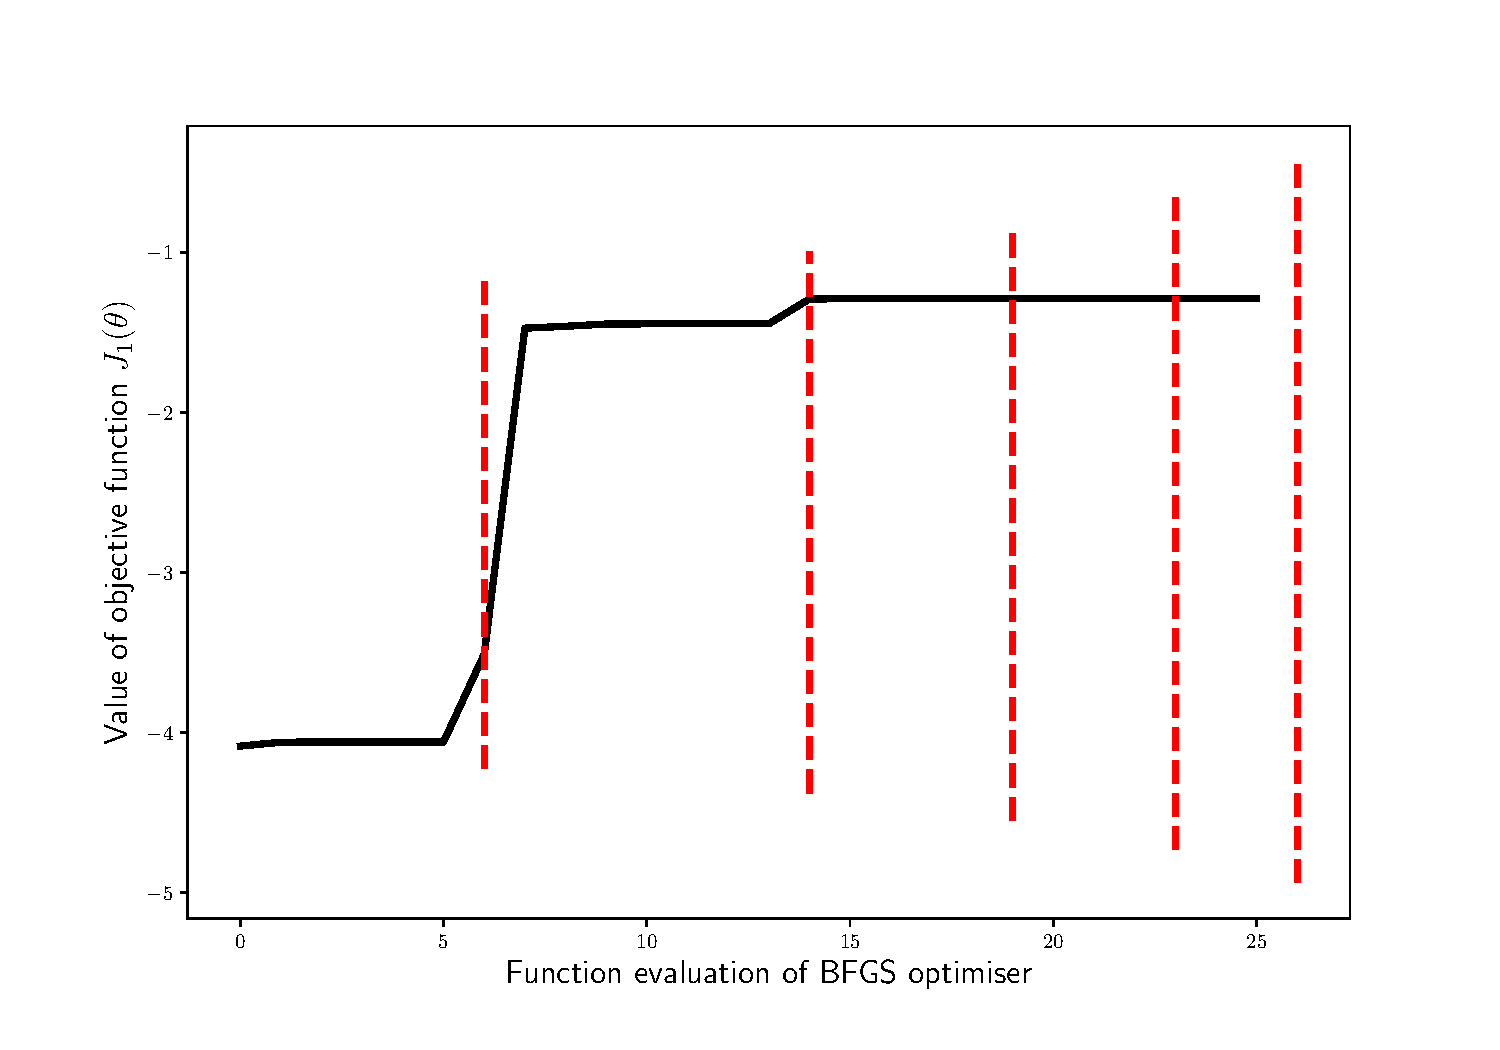
\includegraphics[width = 0.9 \textwidth]{em-loss-curve-mog.pdf}
    \caption{\label{fig:mog-em-loss-curve} EM type algorithm applied to a normalised Mixture of Gaussians model. The red lines indicate when we make the update $q(z|u) = p(z|u; \theta_k)$ where $\theta_k$ is the value of $\theta$ at that point during the optimisation.}.
\end{figure}

\afterpage{
    \thispagestyle{empty}
    \begin{figure}[ht]
      \centering
      \caption{\label{fig:normalised-mog} EM type algorithm applied to a normalised Mixture of Gaussians model. The notation $J^1_{\theta_k}$ in the legends refers to the variational lower bound of the NCE objective function where the variational distribution $q(z|u)$ is set to $p(z|u; \theta_k)$}.
      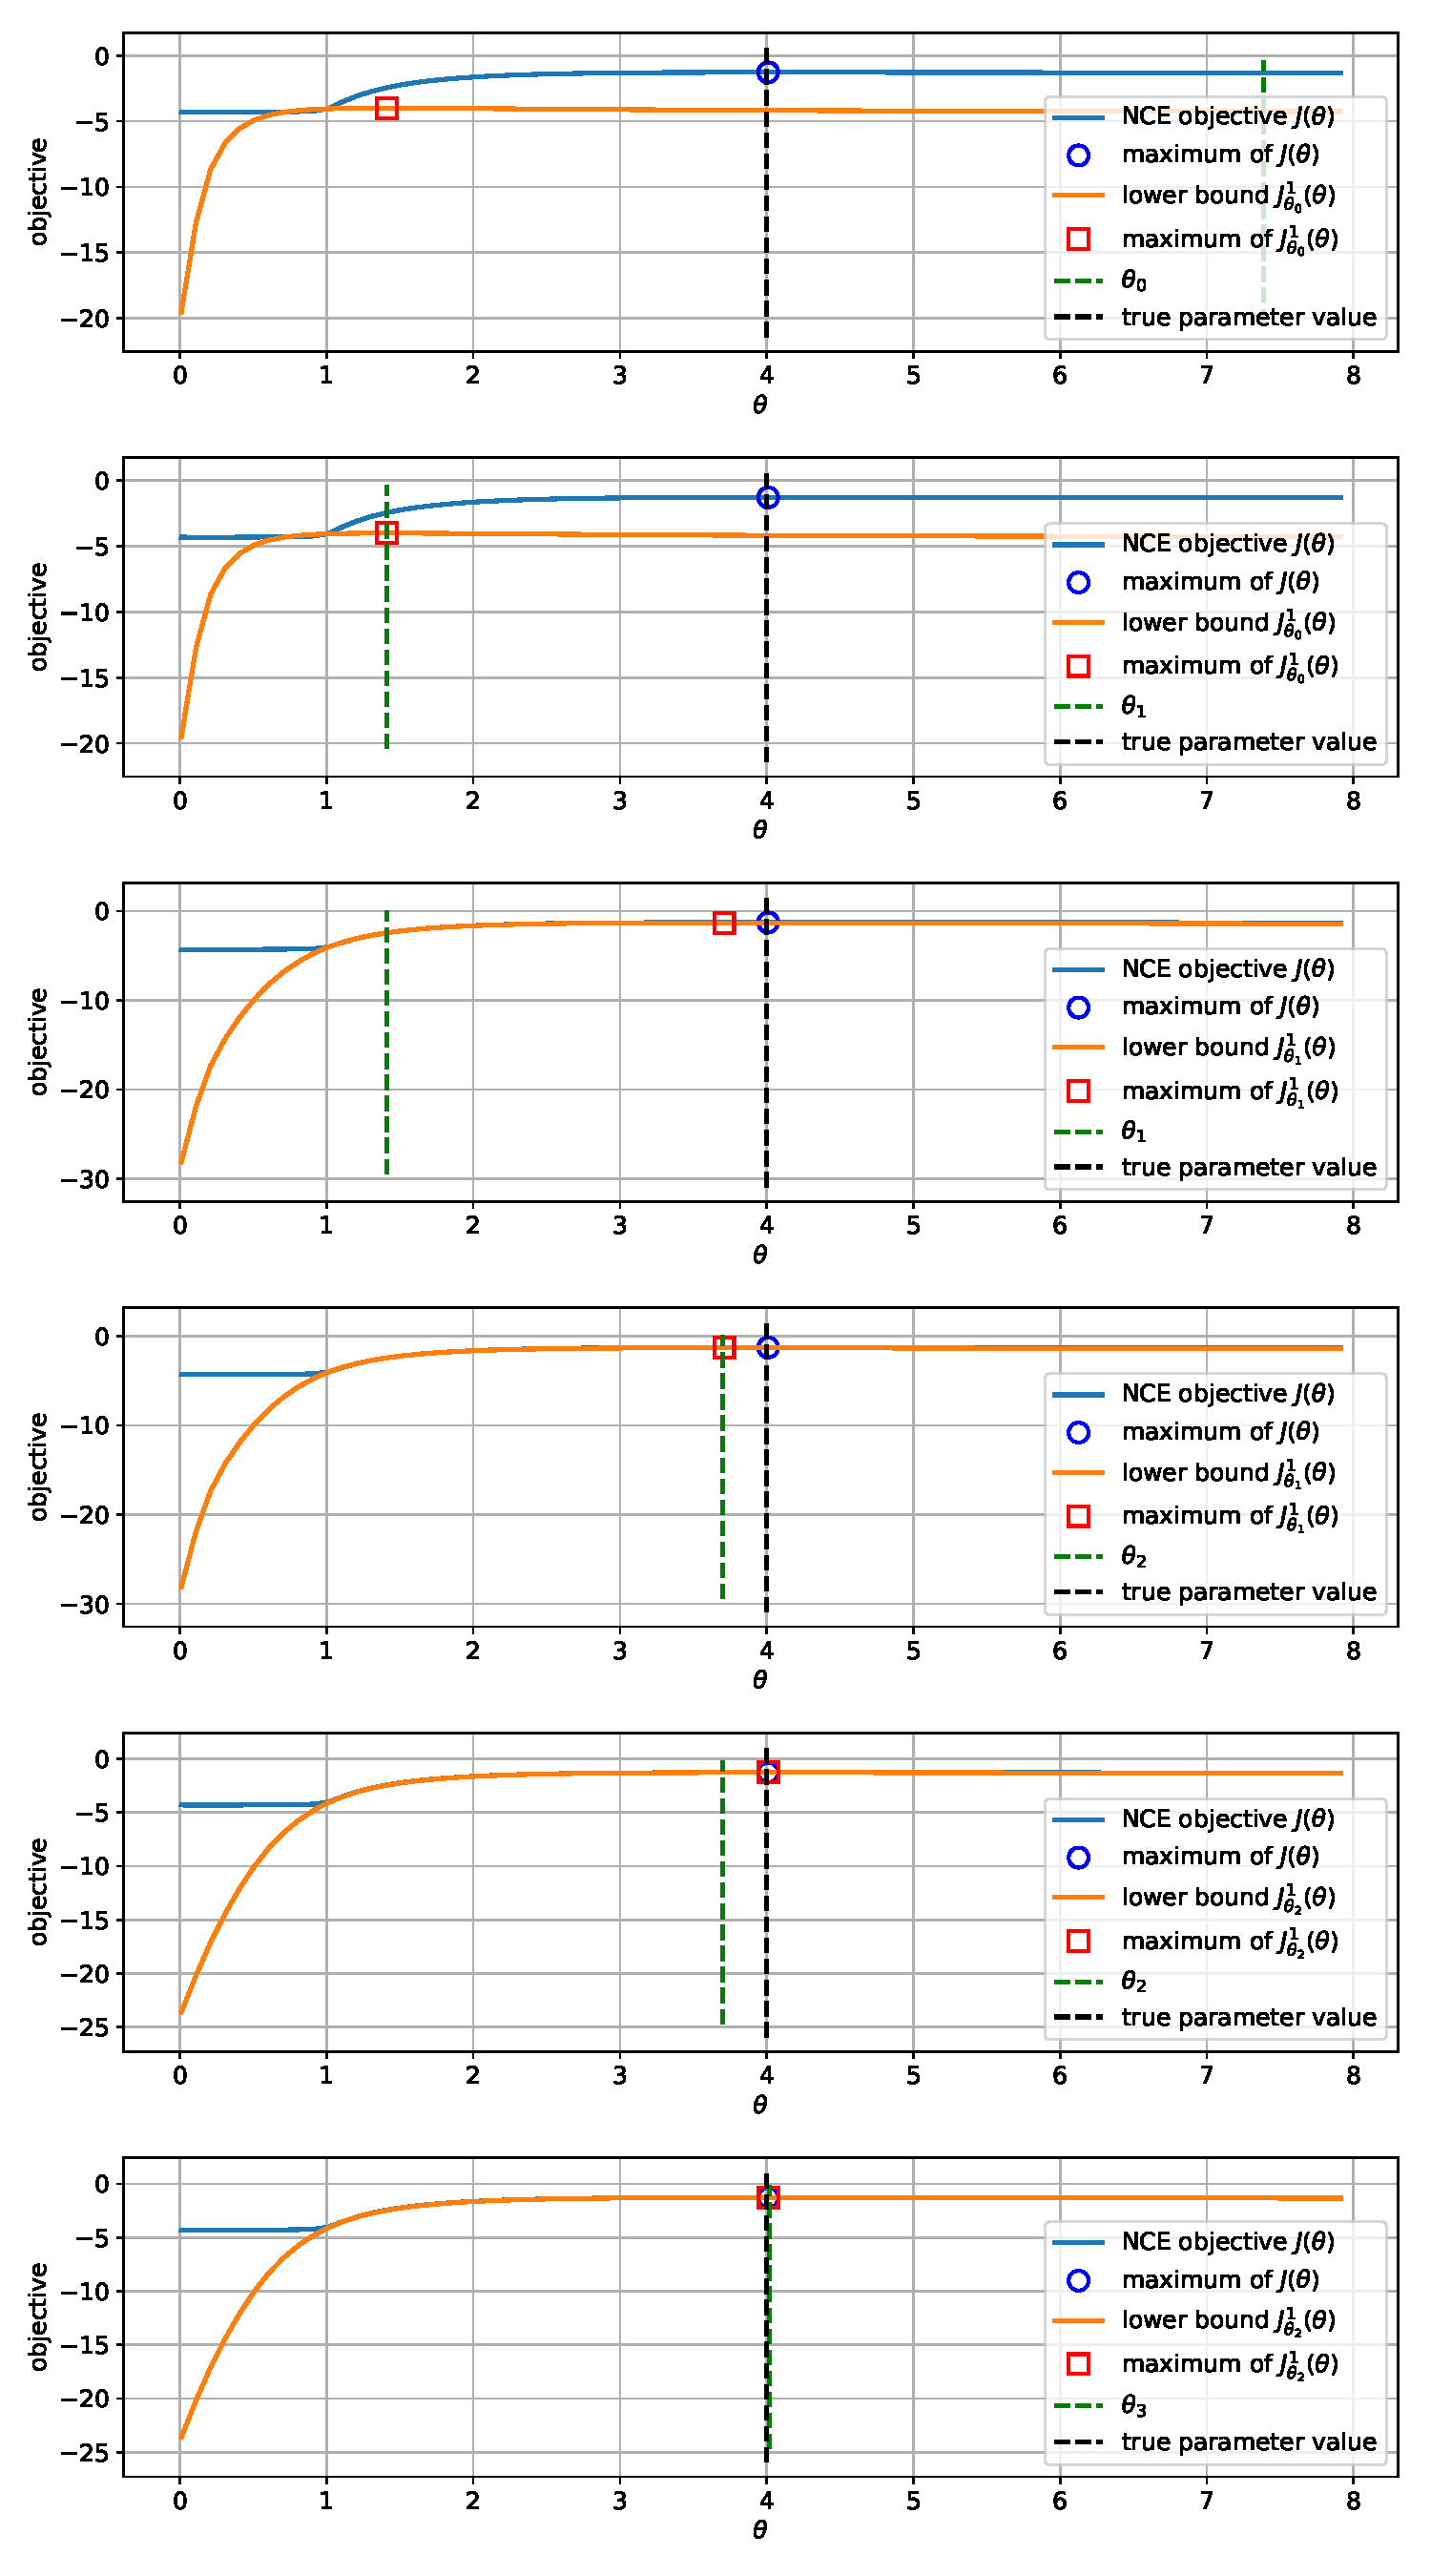
\includegraphics[width = 0.9 \textwidth]{variational-em.pdf}
    \end{figure}
    \clearpage
}

\newpage
\noindent \textbf{The unnormalised case}

We would like to modify the MoG given in equation \ref{eq:mog standard} to obtain an unnormalised family. An obvious candidate is:
\begin{equation}
\phi(u, z; \theta, c) = e^{-c} \left( (1-z) e^{-\frac{u^2}{2 \theta^2}} + z e^{-\frac{u^2}{2 \sigma_1^2}} \right)
\label{eq:mog unnormalised}
\end{equation}
where $e^{-c}$ is a scaling parameter needed for NCE, as discussed at the end of section \ref{sec:nce}. It is important to note that the usual MoG family in equation \ref{eq:mog standard} is \emph{not} nested within unnormalised family in equation \ref{eq:mog unnormalised}. We can see this more easily by normalising \ref{eq:mog unnormalised}, giving us:
\begin{equation}
    \pnorm(u, z, \theta) = (1-z)\frac{\theta}{\theta + \sigma_1} \mathcal{N}(u; 0, \theta) +
                     z\frac{\sigma_1}{\theta + \sigma_1} \mathcal{N}(u; 0, \sigma_1)
\label{eq:mog normalised version of unnormalised}
\end{equation}
We see that the parameter $\theta$ of the unnormalised MoG controls both the width of the first component and its scale relative to the second component. 

As before, fix $\sigma_1 = 1$ and $\Hat{\theta}=4$. Using equation \ref{eq:mog normalised version of unnormalised}, we can easily sample synthetic data from our unnormalised model $\phi$ (still under the assumption that $z \sim \mathcal{B}er(\frac{1}{2})$). To do so, we simply sample $w \sim \mathcal{B}er(\frac{\sigma_1}{\theta + \sigma_1})$ and then sample $\{x_1, ..., x_i\}$ data points:
\[
    x_i \sim \left\{\begin{array}{lr}
        \mathcal{N}(u; 0, \theta), & \text{if } w = 0\\
         \mathcal{N}(u; 0, \sigma_1), & \text{if } w = 1
        \end{array}
\]
Using this synthetic data, we proceed as before, using an EM algorithm to learn the parameter $\theta$. Visualising learning is less straightforward now that our parameter set is 2-dimensional, but we can compare the contour plot of the true NCE objective function against the lower bound obtained at the end of learning. This is given in figure \ref{fig:unnormalised mog contour}. We see that the algorithm converges to the correct value of $\theta$, and correct normalising constant.

\afterpage{
    \thispagestyle{empty}
    \begin{figure}[ht]
    \centering
    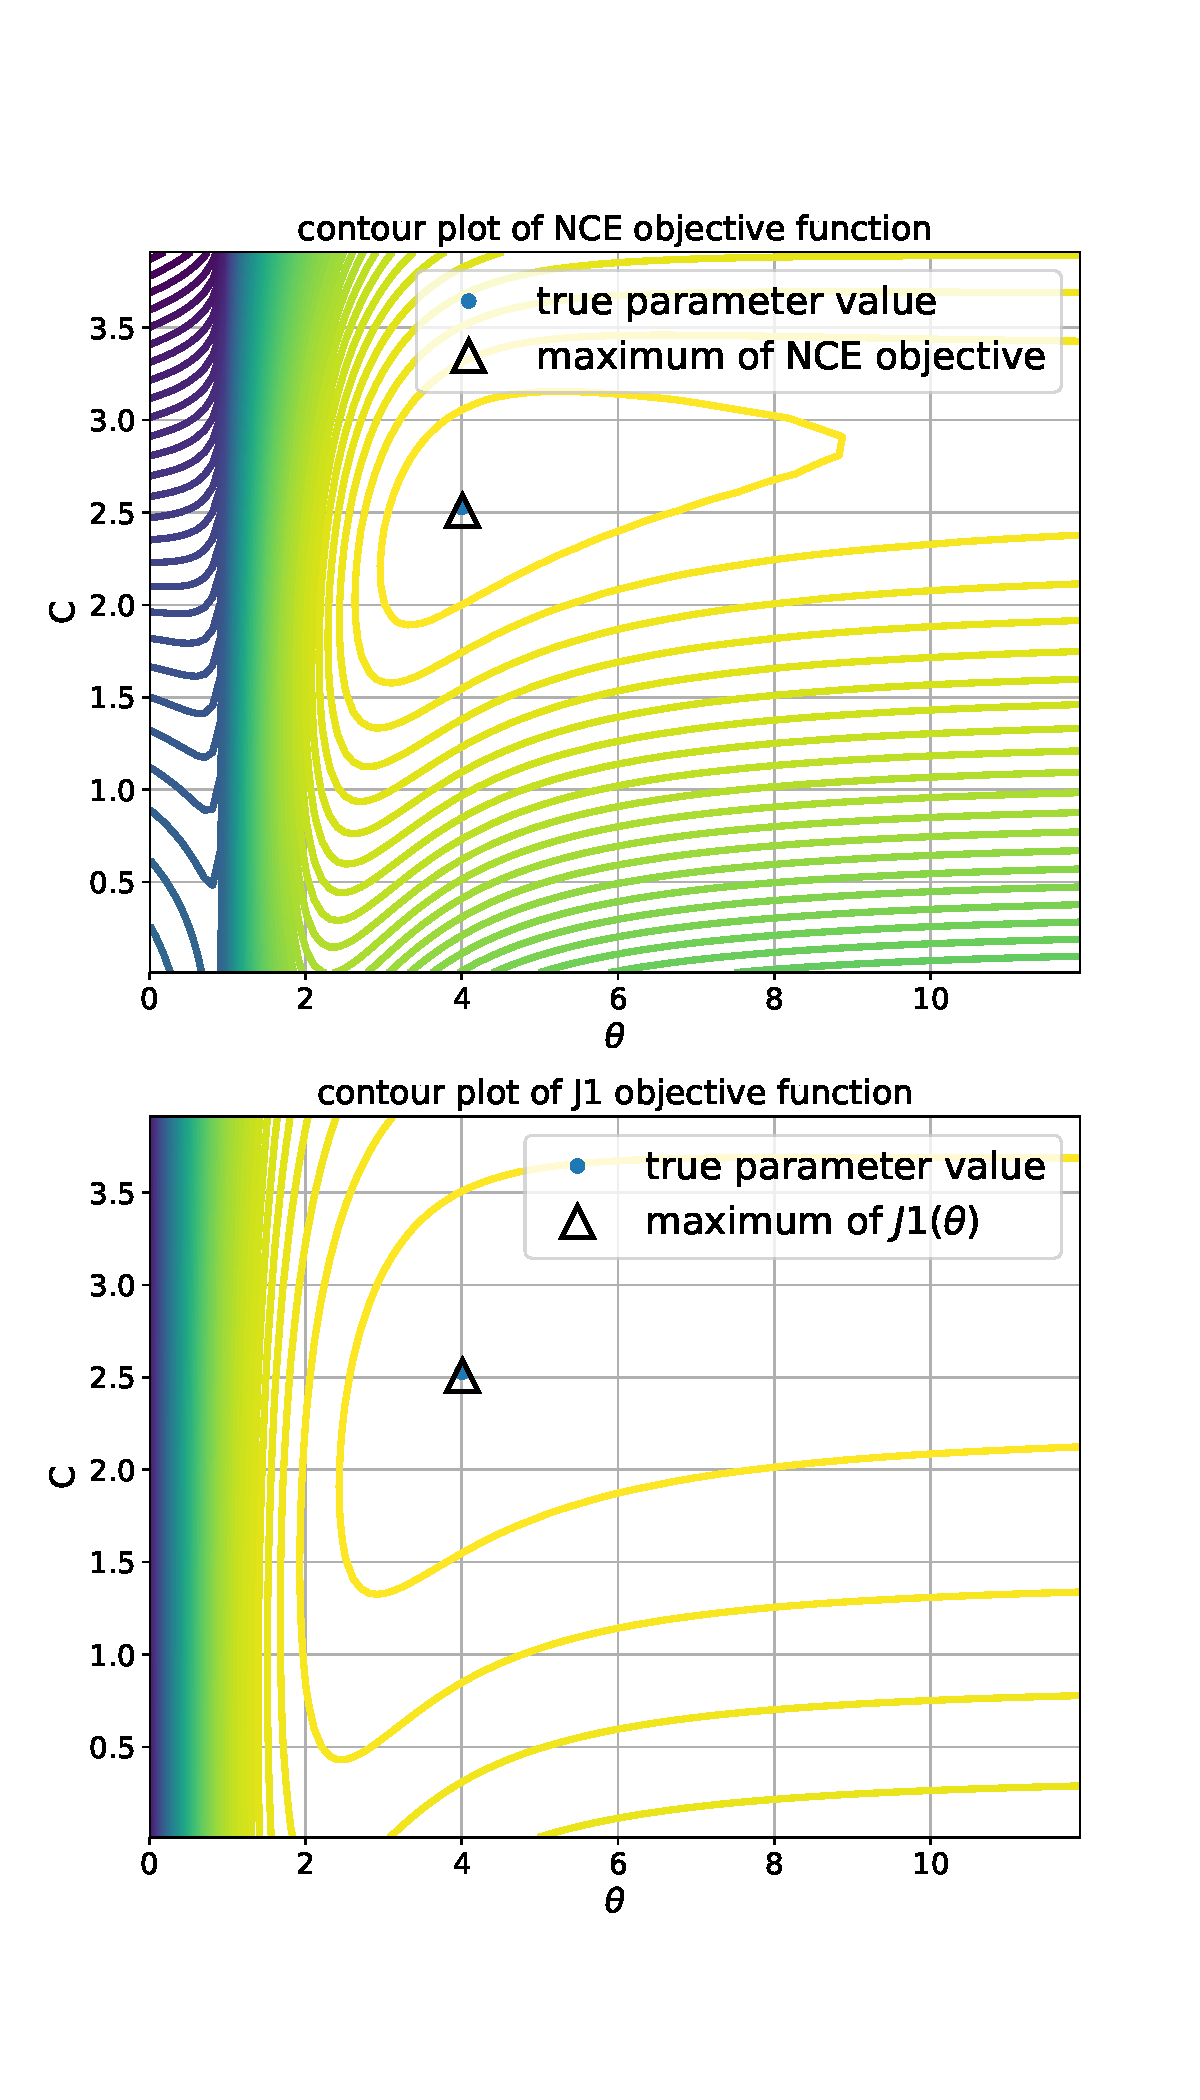
\includegraphics[width = 0.8 \textwidth]{unnormalised-mog-countour.pdf}
    \caption{\label{fig:unnormalised mog contour} contour plot of true NCE objective function compared to the variational lower bound, where we have set the variational distribution $q(z|u)$ to be the posterior $p(z|u; \tilde{\theta})$, where $\tilde{\theta}$ is our final estimate obtained after optimisation. The vertical axis corresponds to $c$, the scaling parameter.}
    \end{figure}
    \clearpage
}


\subsection{Restricted Boltzmann Machine}
\label{sec:rbm}

Due to time limitations, this section is largely incomplete. Obviously a proper introduction to the RBM needs to be given, along with equations, as was done in the case of the Mixture of Gaussians.

Nevertheless, it seems worthwhile documenting my progress on this section. I have applied variational NCE to a low-dimensional RBM, and have early indicators that the method works. Namely, the log-likelihood of the trained model is close to the log-likelihood of the data generating distribution.

The next steps involve implementing contrastive divergence so that I have a baseline to rigoursly compare variational NCE against. I can then see how well the method scales with model complexity compared to the baseline.

\section{Present conclusions and remaining work}

Our goal in this preliminary version of the thesis was twofold. Firstly, to give an exposition of an extension to noise-contrastive estimation which applies to unnormalised models with latent variables. Secondly, to evaluate the performance of this new method in the context of two models: a simple unnormalised mixture of gaussians, and a Restricted Boltzmann Machine.

Both evaluations are ongoing, so it is not yet clear how the new method compares to others, such as contrastive divergence. Nevertheless, current results demonstrate that the method can be successfully used for density estimation, at least on simple problems. The remainder of the thesis will need to critically assess how the method scales with model complexity, sample size and diversity of data generating distributions.

In terms of theory, there is also plenty of work remaining. In particular, we have discussed how it would be interesting to explore the convergence properties of this new estimator, as well as performing a mathematical comparison with contrastive divergence. Finally, once the investigation of RBMs is complete, the next logical step is to investigate models with intractable posteriors that are hard to sample from, since our estimation method can, in theory, work in this setting, whilst contrastive divergence cannot.




\newpage
\section{Appendix}
\subsection{Variational lower bound J1($\theta$)}
\label{sec:appendix derivation of J1}
\label{lower bound}
\begin{align}
  - \log [1+\nu \exp(-h(\u;\thetab))] & =  - \log \left[1+\nu \exp \left(- \log \frac{\pnn(\u;\thetab)}{\pnoise(\u)}\right) \right]\\
  & =  - \log \left[1+\nu \exp \left( \log \frac{\pnoise(\u)}{\pnn(\u;\thetab)}\right) \right]\\
  & =  - \log \left[1+\nu  \frac{\pnoise(\u)}{\pnn(\u;\thetab)} \right] 
\end{align}
Let further
\begin{equation}
  r(\u;\thetab) = \exp(h(\u; \thetab)) = \frac{\pnn(\u;\thetab)}{\pnoise(\u)}
\end{equation}
and
\begin{equation}
  g(r) = -\log \left(1+\nu \frac{1}{r} \right),
\end{equation}
we then obtain
\begin{equation}
  - \log [1+\nu \exp(-h(\u;\thetab))]  = g(r(\u; \thetab)).
\end{equation}
The first derivative of $g$ with respect to $r$ is
\begin{align}
\dod{g}{r} &= \frac{-1}{1+\nu \frac{1}{r}}\frac{-\nu}{r^2}\\
&= \frac{\nu}{r^2+\nu r}
\end{align}
The second derivative of $g$ with respect to $r$ is thus
\begin{align}
\dod[2]{g}{r} &= -\nu \frac{2r +\nu}{(r^2+\nu r)^2},
\end{align}
which is always negative for $r>0$. The function $g(r)$ is thus concave.

We now introduce an auxiliary distribution $q_u(\z)$ over $\z$ and write
\begin{align}
  \pnn(\u; \thetab) &= \int \pnn(\u, \z;\thetab) \dif \z\\
  & = \int q_u(\z) \frac{\pnn(\u,\z; \thetab)}{q_u(\z)} \dif \z\\
  & = \E_{\z \sim q_u} \left[\frac{\pnn(\u,\z; \thetab)}{q_u(\z)}\right]
\end{align}
This corresponds to estimating $\pnn(\u,\thetab)$ by importance sampling. The subscript for $q_u(\z)$ is meant to indicate that we can use different auxiliary distributions for different values of $\u$.

We can thus write $r(\u; \thetab)$ as
\begin{align}
  r(\u;\thetab) &= \frac{1}{\pnoise(\u)}  \E_{\z \sim q_u} \left[\frac{\pnn(\u,\z; \thetab)}{q_u(\z)}\right] \\
  & =  \E_{\z \sim q_u} \left[\frac{\pnn(\u,\z; \thetab)} {q_u(\z)\pnoise(\u)} \right]
\end{align}
and since $g$ is concave, we have
\begin{align}
  - \log [1+\nu \exp(-h(\u;\thetab))]  &= g(r(\u; \thetab)) \\
  & = g\left(\E_{\z \sim q_u} \left[\frac{\pnn(\u,\z; \thetab)} {q_u(\z)\pnoise(\u)} \right]\right)\\
  & \ge \E_{\z \sim q_u} g\left( \frac{\pnn(\u,\z; \thetab)} {q_u(\z)\pnoise(\u)} \right).
\end{align}
With the definition of $g$, we thus obtain
\begin{equation}
  - \log [1+\nu \exp(-h(\u;\thetab))]  \ge -\E_{\z \sim q_u} \log \left[1+\nu \frac{q_u(\z)\pnoise(\u)}{\pnn(\u,\z; \thetab)}\right].
\end{equation}
We now plug this relation into the definition of $J(\thetab)$:
\begin{align}
  J(\thetab)  &= - \Ex  \log \left[1+\nu \exp(-h(\x;\thetab))\right] - \nu \Ey \log \left[1+1/\nu \exp(h(\y;\thetab))\right]\\
  & \ge  -\Ex \E_{\z \sim q(\z|\x)} \log \left[1+\nu \frac{q(\z|\x)\pnoise(\x)}{\pnn(\x,\z; \thetab)}\right] -  \nu \Ey \log \left[1+1/\nu \exp(h(\y;\thetab))\right] \\
    &\geq -\Ex \E_{\z \sim q(\z|\x)} \log \left[1+\nu \frac{q(\z|\x)\pnoise(\x)}{\pnn(\x,\z; \thetab)}\right] -  \nu \Ey \log \left[1+\frac{1}{\nu} \E_{\z \sim q(\z | \y)} \left[\frac{\pnn(\y,\z; \thetab)} {q(\z | \y)\pnoise(\y)} \right]  \right].
\end{align}


\subsection{Gradient of J1($\theta$)}
\label{sec:appendix grad of J1}
To find the argmax of $J_1(\theta)$, we need to differentiate it. To do so, let us first further reduce the notational burden, by writing:

\begin{align}
J_1(\theta) & =  
              \color{red}{ - \mathbb{E}_{x} \mathbb{E}_{z \sim q_k} \left[ \log(\psi_1(x, z; \theta)) \right]} -        \color{blue}{ \nu \mathbb{E}_{y}  \left[  \log(\psi_2(y; \theta)) \right]}
\end{align}
where
\begin{align}
\color{red}{\psi_1(x, z; \theta) = 1 + \frac{\nu}{r(x, z; \theta)}} \\
\color{blue}{\psi_2(y; \theta) = 1 + \frac{1}{\nu} \mathbb{E}_{z \sim q_k}[r(y, z; \theta)]}
\end{align}

Now, let us take derivative with respect to $\theta$:

\begin{align}
\color{red}{ \nabla_{\theta} \log(\psi_1(x, z; \theta))} 
           & = \frac{1}{\psi_1(x, z; \theta)} \nabla_{\theta} \psi_1(x, z; \theta) \\
           & = \frac{1}{\psi_1(x, z; \theta)} \frac{-\nu}{r(x, z; \theta)^2} \nabla_{\theta} r(x, z; \theta) \\
           & = \frac{1}{\psi_1(x, z; \theta)} \frac{-\nu}{r(x, z; \theta)^2} \frac{\nabla_{\theta} \phi(x, z; \theta)}{q_k(z \ | \ x)p_y(x)}
\end{align}

Hence, we need:

\begin{align}
\nabla_{\theta} \phi(x, z; \theta) & = \nabla_{\theta} \exp ( \log ( \phi(x, z; \theta) ) ) \\
          & = \left[ \nabla_{\theta} \log(\phi(x, z; \theta)) \right] \exp ( \log ( \phi(x, z; \theta) ) )\\
          & = \left[ \nabla_{\theta} \log(\phi(x, z; \theta)) \right] \phi(x, z; \theta) 
\end{align}

Plugging this back in, we get:

\begin{align}
\color{red}{ \nabla_{\theta} \log(\psi_1(x, z; \theta))} 
    & = \frac{1}{\psi_1(x, z; \theta)} 
        \frac{-\nu}{r(x, z; \theta)^2} 
        \frac{\left[ \nabla_{\theta} \log(\phi(x, z; \theta)) \right] \phi(x, z; \theta)}{q_k(z \ | \ x)p_y(x)} \\
    & = \frac{1}{\psi_1(x, z; \theta)} 
        \frac{-\nu}{r(x, z; \theta)} 
        \left[ \nabla_{\theta} \log(\phi(x, z; \theta)) \right] \\
    & = \color{red}{- \frac{\psi_1(x, z; \theta) - 1}{\psi_1(x, z; \theta)} 
        \left[ \nabla_{\theta} \log(\phi(x, z; \theta)) \right]} \\
\end{align}

Where in the final line we used the fact that $\color{red}{\psi_1(x, z; \theta) - 1 = \frac{\nu}{r(x, z; \theta)}}$.

Now we find the derivative of the second (blue) term of $J_1^K(\theta)$. Recalling that $\color{blue}{\psi_2(y; \theta) = 1 + \frac{1}{\nu} \mathbb{E}_{z \sim q_k}[r(y, z; \theta)]}$, we have:

\begin{align}
\color{blue}{\nabla_{\theta} \log(\psi_2(y; \theta))}
    & = \frac{1}{\psi_2(y; \theta)} \nabla_{\theta} \psi_2(y; \theta) \\
    & = \frac{1}{\psi_2(y; \theta)} 
        \frac{1}{\nu} \mathbb{E}_{z \sim q_k} 
        \left[ \frac{\nabla_{\theta} \phi(y, z; \theta)}{q_k(z \ | \ y)p_y(y)} \right] \\  
    & = \color{blue}{\frac{1}{\nu} 
        \frac{1}{\psi_2(y; \theta)} 
        \mathbb{E}_{z \sim q_k} \left[ r(y, z; \theta) \left[ \nabla_{\theta} \log(\phi(y, z; \theta)) \right] \right]} \\
\end{align}

Putting this all together, we arrive at: 

\begin{align}
\nabla_{\theta}(J_1^k(\theta)) & =  
    \color{red}{ \mathbb{E}_{x} \mathbb{E}_{z \sim q_k} \frac{\psi_1(x, z; \theta) - 1}{\psi_1(x, z; \theta)} 
                \left[ \nabla_{\theta} \log(\phi(x, z; \theta)) \right]} \\
    &\color{blue}{ - \mathbb{E}_y
                 \frac{1}{\psi_2(y; \theta)} 
                \mathbb{E}_{z \sim q_k} \left[ r(y, z; \theta) \left[ \nabla_{\theta} \log(\phi(y, z; \theta)) \right] \right]} \\
\end{align}

Where (to remind ourselves yet again): 
\begin{align}
\color{red}{\psi_1(x, z; \theta) = 1 + \frac{\nu}{r(x, z; \theta)}} \\
\color{blue}{\psi_2(y; \theta) = 1 + \frac{1}{\nu} \mathbb{E}_{z \sim q_k}[r(y, z; \theta)]}
\end{align}

\newpage
\bibliographystyle{plainnat}
\bibliography{interim_report.bib}

\end{document}  
